\section{Background}
In this paper, we use objects to denote data points like images or texts. 
Given a matrix $\bfX$, we use $\bfX_i$ to denote its $i$-th row, and $\bfX_{i,j}$ to denote its $(i,j)$-th entry. Same holds for matrices like $\bfW_\bfX$, where we use $\bfW_{\bfX,i}$ and $\bfW_{\bfX,i,j}$, respectively. 


\subsection{Contrastive learning: SimCLR}
Given a query object $\mathbf{q}\in \cX$, 
\textbf{one} similar object $\mathbf{p}_1$ for $\mathbf{q}$, and $N-1$ other objects $\{\mathbf{p}_i\}_{i=2}^{N}$, 
SimCLR finds a function $f$ (usually a neural network) that maps these objects to $\cZ$, to minimize the InfoNCE loss of $\mathbf{q}$:
\begin{equation}
\label{eqn:infonce}
\mathcal{L}(\mathbf{q}, \mathbf{p}_1, \{\mathbf{p}_i\}_{i=2}^{N})=-\log \frac{\exp(\tsim(f(\mathbf{q}), f(\mathbf{p}_1))/\tau)}{\sum_{i=1}^N
\exp(\tsim(f(\mathbf{q}), f(\mathbf{p}_i))/\tau)
}
\end{equation}
Here, the actual loss of $f$ takes the summation over different $\mathbf{q}$, and $\tau$ is a temperature hyperparameter. 
The $\tsim(\bfZ_i, \bfZ_j)$ function measures the similarity between $\bfZ_i, \bfZ_j$ in $\cZ$, and is commonly  defined as $\tsim(\bfZ_i,  \bfZ_j)=\frac{\bfZ_i^\top \bfZ_j }{\|\bfZ_i\|\|\bfZ_j\|} $, 
or $\bfZ_i^\top \bfZ_j$, 
or $- \|\bfZ_i- \bfZ_j\|^2/2 $. 
In this paper, we consider the case that $\cZ$ is the unit sphere, i.e., $\|\bfZ_i\|=\|\bfZ_j\|=1$. 
This is because both SimCLR and CLIP have a normalization step in the implementation~~\citep{chen2020simple, radford2021learning}.
Hence, $
\frac{\bfZ_i^\top \bfZ_j}{\|\bfZ_i\|\|\bfZ_j\|}=
\bfZ_i^\top \bfZ_j$, and 
\begin{equation}
\label{eqn:sim_equivalence}
-\|\bfZ_i- \bfZ_j\|^2/2= -\bfZ_i^2/2 - \bfZ_j^2/2 + \bfZ_i^\top \bfZ_j = 
-1+\bfZ_i^\top \bfZ_j. 
\end{equation}
Therefore, these losses are the same up to a constant. 

\subsection{Multi-modal learning: CLIP}
CLIP~~\citep{radford2021learning} is a multi-modal model  with a dataset containing millions of (image, text) pairs. 
During pretraining, for each batch of $N$ pairs of data points, CLIP uses an image encoder and a text encoder to get $N$ pairs of embeddings, and use the InfoNCE loss to compute the correct $N$ pairs out of  $N\times N$ possible connections. Specifically, given an image $\ai$, we compare the its matching score of the paired text $\bi$, with the matching scores of other $N-1$ texts $\{\mathbf{b}_j\}_{j\neq i}$, using the loss $\ell(\ai, \bi, \{\mathbf{b}_j\}_{j\neq i})$ defined in Eqn.~(\ref{eqn:infonce}) by setting $\tsim(\bfZ_i,  \bfZ_j)=\frac{\bfZ_i^\top \bfZ_j }{\|\bfZ_i\|\|\bfZ_j\|} $.


One can define the loss similarly for text, and the actual loss of the embedding network $f$ takes the summation over all the images and  texts. 



\subsection{Reproducing Kernel Hilbert Space}
\label{sec:rkhs}
Given two objects $\bfZ_i, \bfZ_j 
\in \cZ$, consider a feature map $\varphi: \cZ\rightarrow \cH$, where the feature space $\cH$ is usually much larger than $\cZ$. We may define a kernel $k$ that measures the similarity of $\bfZ_i, \bfZ_j$ as $k(\bfZ_i, \bfZ_j)\triangleq \langle \varphi(\bfZ_i), \varphi(\bfZ_j)\rangle_\cH$, i.e., the inner product between the two objects after mapping them to the feature space. For any vector $h\in \cH$, it also corresponds to a function $h(\cdot): \cZ\rightarrow \mathbb{R}$, defined as $h(\bfZ_i)=\langle h, \varphi(\bfZ_i)\rangle_\cH$. Specifically,
$\varphi(\bfZ_j)$ as a vector in $\cH$ represents the function $k(\cdot, \bfZ_j): \cZ\rightarrow \mathbb{R}$, because for any $\bfZ_i\in \cZ$, we have $k(\bfZ_i, \bfZ_j)=\langle \varphi(\bfZ_i), \varphi(\bfZ_j)\rangle_\cH$. Formally, we have:
\begin{definition}[Reproducing kernel Hilbert space]
\label{def:rkhs}
Let $\cH$ be a Hilbert space of $\mathbb{R}$-valued functions defined on a non-empty set $\cZ$. A function $k:\cZ\times \cZ \rightarrow \mathbb{R}$ is called a reproducing kernel of $\cH$, and $\cH$ is a
reproducing kernel Hilbert space, if $k$ satisfies
\begin{itemize}[parsep=0cm, topsep=0cm]
    \item $\forall \bfZ_i\in \cZ, k(\cdot, \bfZ_i)\in \cH$,
    \item $\forall \bfZ_i\in \cZ, \forall h\in \cH, \langle h, k(\cdot, \bfZ_i)\rangle_\cH=h(\bfZ_i).$
\end{itemize}    
\end{definition}

We focus on the translation-invariant kernel in our paper, where the kernel $k(\bfZ_i,\bfZ_j)$ can always be written as $k'(\bfZ_i-\bfZ_j)$ for $k'\in \cZ\rightarrow \mathbb{R}$. The Moore–Aronszajn's theorem states that if $k$ is a symmetric, positive definite kernel on $\cZ$, there is a unique Hilbert space of functions $\cH$ on $\cZ$ for which $k$ is a reproducing kernel.

For instance, the Gaussian kernel is a symmetric, positive definite kernel that yields an RKHS with infinite dimensions. One of the advantages of a reproducing kernel is that the similarity can be computed directly in $\cZ$ without using the feature map to go to the potentially infinite dimensional Hilbert space. However, a reproducing kernel's similarity structure should ideally align with the semantic meanings of specific tasks. For example, it is unlikely to calculate the semantic similarity of two images directly using a predefined reproducing kernel in the pixel space.

Consequently, we ask if it is possible to find an embedding function $f:\cX\rightarrow \cZ$, where $\cZ$ can compute the similarity of two objects in $\cX$ with a predefined kernel function, i.e., whether $\bfK_\bfZ$ matches with $\bfpi$ in Figure~\ref{fig:illustration}. 
In other words, we hope to map
the objects to a space where the semantic similarity in $\cX$ is naturally embedded. This is the starting point of our paper.


\subsection{Markov random field}
 In this subsection, we present the framework (without proofs) of MRF for dimension reduction~~\citep{van2022probabilistic}. 
We have modified some definitions and lemmas for our learning scenarios, and the readers may check the paper for more details on this framework. 

Consider $n$ objects $\bfZ=[\bfZ_1, \cdots, \bfZ_n]$ in $\mathcal{Z}$. We use a symmetric and translation invariant kernel  $k: \cZ\rightarrow \mathbb{R}_+$ to represent the similarities in $\cZ$, where
symmetric means $k(\mathbf{x})=k(-\mathbf{x})$. Given $\bfZ$ and $k$, 
we define the gram matrix  as $\bfK_\bfZ\triangleq (k(\bfZ_i-\bfZ_j))_{(i,j)\in [n]^2}$, which is also the adjacency matrix representing the similarities of objects in $\bfZ$. 

As discussed previously, directly comparing $\bfK_\bfZ$ and $\bfpi$ can be difficult, so we treat them as MRFs and compare the induced probability distributions on subgraphs instead.
In our paper, 
subgraphs are directed unweighted graphs from the set $S_\bfW\triangleq 
\{\bfW\in \{0,1\}^{n\times n} ~|~ \forall (i,j)\in [n]^2, \bfW_{i,i}=0\}$. 
The distribution of $\bfW$ is generally defined as follows. 

\begin{definition}[Distribution of $\bfW$]
\label{def:prior_w}
Let $\bfpi\in \mathbb{R}_+^{n\times n}$, we define the distribution $
\mathbb{P} (\bfW;\bfpi) \propto 
\Omega(\bfW) 
\Pi_{(i,j)\in [n]^2} \bfpi_{i,j}^{\bfW_{i,j}}$, 
where
$\Omega(\bfW)\triangleq \Pi_i \mathbb{I}_{\sum_j \bfW_{i,j}=1}$.
\end{definition}


\begin{figure*}
\begin{center}


\tikzset{every picture/.style={line width=0.75pt}} %set default line width to 0.75pt        

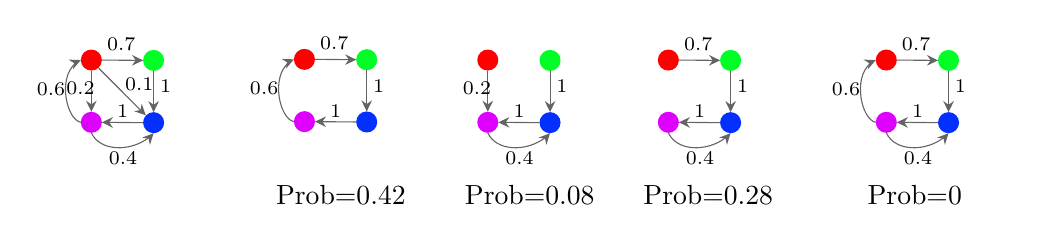
\begin{tikzpicture}[x=0.75pt,y=0.75pt,yscale=-1,xscale=1]
%uncomment if require: \path (0,300); %set diagram left start at 0, and has height of 300

%Shape: Circle [id:dp6680159379724935] 
\draw  [draw opacity=0][fill={rgb, 255:red, 255; green, 0; blue, 0 }  ,fill opacity=1 ] (210,135.27) .. controls (210,132.47) and (212.27,130.2) .. (215.07,130.2) .. controls (217.86,130.2) and (220.13,132.47) .. (220.13,135.27) .. controls (220.13,138.06) and (217.86,140.33) .. (215.07,140.33) .. controls (212.27,140.33) and (210,138.06) .. (210,135.27) -- cycle ;
%Shape: Circle [id:dp2937575833870516] 
\draw  [draw opacity=0][fill={rgb, 255:red, 0; green, 255; blue, 38 }  ,fill opacity=1 ] (240,135.43) .. controls (240,132.64) and (242.27,130.37) .. (245.07,130.37) .. controls (247.86,130.37) and (250.13,132.64) .. (250.13,135.43) .. controls (250.13,138.23) and (247.86,140.5) .. (245.07,140.5) .. controls (242.27,140.5) and (240,138.23) .. (240,135.43) -- cycle ;
%Shape: Circle [id:dp5400820274117357] 
\draw  [draw opacity=0][fill={rgb, 255:red, 3; green, 47; blue, 255 }  ,fill opacity=1 ] (240,165.43) .. controls (240,162.64) and (242.27,160.37) .. (245.07,160.37) .. controls (247.86,160.37) and (250.13,162.64) .. (250.13,165.43) .. controls (250.13,168.23) and (247.86,170.5) .. (245.07,170.5) .. controls (242.27,170.5) and (240,168.23) .. (240,165.43) -- cycle ;
%Shape: Circle [id:dp012766690091095434] 
\draw  [draw opacity=0][fill={rgb, 255:red, 222; green, 0; blue, 255 }  ,fill opacity=1 ] (210,165.27) .. controls (210,162.47) and (212.27,160.2) .. (215.07,160.2) .. controls (217.86,160.2) and (220.13,162.47) .. (220.13,165.27) .. controls (220.13,168.06) and (217.86,170.33) .. (215.07,170.33) .. controls (212.27,170.33) and (210,168.06) .. (210,165.27) -- cycle ;
%Straight Lines [id:da5536414406911649] 
\draw [color={rgb, 255:red, 100; green, 100; blue, 100 }  ,draw opacity=1 ]   (220.13,135.27) -- (237,135.41) ;
\draw [shift={(240,135.43)}, rotate = 180.48] [fill={rgb, 255:red, 100; green, 100; blue, 100 }  ,fill opacity=1 ][line width=0.08]  [draw opacity=0] (5.36,-2.57) -- (0,0) -- (5.36,2.57) -- (3.56,0) -- cycle    ;
%Straight Lines [id:da8056930605061887] 
\draw [color={rgb, 255:red, 100; green, 100; blue, 100 }  ,draw opacity=1 ]   (223.13,165.29) -- (240,165.43) ;
\draw [shift={(220.13,165.27)}, rotate = 0.48] [fill={rgb, 255:red, 100; green, 100; blue, 100 }  ,fill opacity=1 ][line width=0.08]  [draw opacity=0] (5.36,-2.57) -- (0,0) -- (5.36,2.57) -- (3.56,0) -- cycle    ;
%Straight Lines [id:da5796955635821128] 
\draw [color={rgb, 255:red, 100; green, 100; blue, 100 }  ,draw opacity=1 ]   (215.07,140.33) -- (215.07,157.2) ;
\draw [shift={(215.07,160.2)}, rotate = 270] [fill={rgb, 255:red, 100; green, 100; blue, 100 }  ,fill opacity=1 ][line width=0.08]  [draw opacity=0] (5.36,-2.57) -- (0,0) -- (5.36,2.57) -- (3.56,0) -- cycle    ;
%Straight Lines [id:da788839051424455] 
\draw [color={rgb, 255:red, 100; green, 100; blue, 100 }  ,draw opacity=1 ]   (245.07,140.5) -- (245.07,157.37) ;
\draw [shift={(245.07,160.37)}, rotate = 270] [fill={rgb, 255:red, 100; green, 100; blue, 100 }  ,fill opacity=1 ][line width=0.08]  [draw opacity=0] (5.36,-2.57) -- (0,0) -- (5.36,2.57) -- (3.56,0) -- cycle    ;
%Straight Lines [id:da09644761921540357] 
\draw [color={rgb, 255:red, 100; green, 100; blue, 100 }  ,draw opacity=1 ]   (218.63,139.22) -- (239.15,159.76) ;
\draw [shift={(241.27,161.88)}, rotate = 225.04] [fill={rgb, 255:red, 100; green, 100; blue, 100 }  ,fill opacity=1 ][line width=0.08]  [draw opacity=0] (5.36,-2.57) -- (0,0) -- (5.36,2.57) -- (3.56,0) -- cycle    ;
%Curve Lines [id:da6909993804639241] 
\draw [color={rgb, 255:red, 100; green, 100; blue, 100 }  ,draw opacity=1 ]   (207.42,136.86) .. controls (198.7,144.14) and (203.19,163.99) .. (210,165.27) ;
\draw [shift={(210,135.27)}, rotate = 156.35] [fill={rgb, 255:red, 100; green, 100; blue, 100 }  ,fill opacity=1 ][line width=0.08]  [draw opacity=0] (5.36,-2.57) -- (0,0) -- (5.36,2.57) -- (3.56,0) -- cycle    ;
%Curve Lines [id:da43617986234567363] 
\draw [color={rgb, 255:red, 100; green, 100; blue, 100 }  ,draw opacity=1 ]   (215.07,170.33) .. controls (219.24,179.43) and (233.96,179.59) .. (242.88,172.51) ;
\draw [shift={(245.07,170.5)}, rotate = 133.09] [fill={rgb, 255:red, 100; green, 100; blue, 100 }  ,fill opacity=1 ][line width=0.08]  [draw opacity=0] (5.36,-2.57) -- (0,0) -- (5.36,2.57) -- (3.56,0) -- cycle    ;
%Shape: Circle [id:dp9613652888659034] 
\draw  [draw opacity=0][fill={rgb, 255:red, 255; green, 0; blue, 0 }  ,fill opacity=1 ] (312.67,134.93) .. controls (312.67,132.14) and (314.94,129.87) .. (317.73,129.87) .. controls (320.53,129.87) and (322.8,132.14) .. (322.8,134.93) .. controls (322.8,137.73) and (320.53,140) .. (317.73,140) .. controls (314.94,140) and (312.67,137.73) .. (312.67,134.93) -- cycle ;
%Shape: Circle [id:dp4333461787824253] 
\draw  [draw opacity=0][fill={rgb, 255:red, 0; green, 255; blue, 38 }  ,fill opacity=1 ] (342.67,135.1) .. controls (342.67,132.3) and (344.94,130.03) .. (347.73,130.03) .. controls (350.53,130.03) and (352.8,132.3) .. (352.8,135.1) .. controls (352.8,137.9) and (350.53,140.17) .. (347.73,140.17) .. controls (344.94,140.17) and (342.67,137.9) .. (342.67,135.1) -- cycle ;
%Shape: Circle [id:dp03365070392980951] 
\draw  [draw opacity=0][fill={rgb, 255:red, 3; green, 47; blue, 255 }  ,fill opacity=1 ] (342.67,165.1) .. controls (342.67,162.3) and (344.94,160.03) .. (347.73,160.03) .. controls (350.53,160.03) and (352.8,162.3) .. (352.8,165.1) .. controls (352.8,167.9) and (350.53,170.17) .. (347.73,170.17) .. controls (344.94,170.17) and (342.67,167.9) .. (342.67,165.1) -- cycle ;
%Shape: Circle [id:dp9062547154952614] 
\draw  [draw opacity=0][fill={rgb, 255:red, 222; green, 0; blue, 255 }  ,fill opacity=1 ] (312.67,164.93) .. controls (312.67,162.14) and (314.94,159.87) .. (317.73,159.87) .. controls (320.53,159.87) and (322.8,162.14) .. (322.8,164.93) .. controls (322.8,167.73) and (320.53,170) .. (317.73,170) .. controls (314.94,170) and (312.67,167.73) .. (312.67,164.93) -- cycle ;
%Straight Lines [id:da5461621784127331] 
\draw [color={rgb, 255:red, 100; green, 100; blue, 100 }  ,draw opacity=1 ]   (322.8,134.93) -- (339.67,135.07) ;
\draw [shift={(342.67,135.1)}, rotate = 180.48] [fill={rgb, 255:red, 100; green, 100; blue, 100 }  ,fill opacity=1 ][line width=0.08]  [draw opacity=0] (5.36,-2.57) -- (0,0) -- (5.36,2.57) -- (3.56,0) -- cycle    ;
%Straight Lines [id:da09616201897578192] 
\draw [color={rgb, 255:red, 100; green, 100; blue, 100 }  ,draw opacity=1 ]   (325.8,164.96) -- (342.67,165.1) ;
\draw [shift={(322.8,164.93)}, rotate = 0.48] [fill={rgb, 255:red, 100; green, 100; blue, 100 }  ,fill opacity=1 ][line width=0.08]  [draw opacity=0] (5.36,-2.57) -- (0,0) -- (5.36,2.57) -- (3.56,0) -- cycle    ;
%Straight Lines [id:da5502296583487012] 
\draw [color={rgb, 255:red, 100; green, 100; blue, 100 }  ,draw opacity=1 ]   (347.73,140.17) -- (347.73,157.03) ;
\draw [shift={(347.73,160.03)}, rotate = 270] [fill={rgb, 255:red, 100; green, 100; blue, 100 }  ,fill opacity=1 ][line width=0.08]  [draw opacity=0] (5.36,-2.57) -- (0,0) -- (5.36,2.57) -- (3.56,0) -- cycle    ;
%Curve Lines [id:da23324631718484024] 
\draw [color={rgb, 255:red, 100; green, 100; blue, 100 }  ,draw opacity=1 ]   (310.09,136.53) .. controls (301.37,143.81) and (305.86,163.66) .. (312.67,164.93) ;
\draw [shift={(312.67,134.93)}, rotate = 156.35] [fill={rgb, 255:red, 100; green, 100; blue, 100 }  ,fill opacity=1 ][line width=0.08]  [draw opacity=0] (5.36,-2.57) -- (0,0) -- (5.36,2.57) -- (3.56,0) -- cycle    ;
%Shape: Circle [id:dp6818622582337936] 
\draw  [draw opacity=0][fill={rgb, 255:red, 255; green, 0; blue, 0 }  ,fill opacity=1 ] (401,135.27) .. controls (401,132.47) and (403.27,130.2) .. (406.07,130.2) .. controls (408.86,130.2) and (411.13,132.47) .. (411.13,135.27) .. controls (411.13,138.06) and (408.86,140.33) .. (406.07,140.33) .. controls (403.27,140.33) and (401,138.06) .. (401,135.27) -- cycle ;
%Shape: Circle [id:dp06363585140660888] 
\draw  [draw opacity=0][fill={rgb, 255:red, 0; green, 255; blue, 38 }  ,fill opacity=1 ] (431,135.43) .. controls (431,132.64) and (433.27,130.37) .. (436.07,130.37) .. controls (438.86,130.37) and (441.13,132.64) .. (441.13,135.43) .. controls (441.13,138.23) and (438.86,140.5) .. (436.07,140.5) .. controls (433.27,140.5) and (431,138.23) .. (431,135.43) -- cycle ;
%Shape: Circle [id:dp6515401713841082] 
\draw  [draw opacity=0][fill={rgb, 255:red, 3; green, 47; blue, 255 }  ,fill opacity=1 ] (431,165.43) .. controls (431,162.64) and (433.27,160.37) .. (436.07,160.37) .. controls (438.86,160.37) and (441.13,162.64) .. (441.13,165.43) .. controls (441.13,168.23) and (438.86,170.5) .. (436.07,170.5) .. controls (433.27,170.5) and (431,168.23) .. (431,165.43) -- cycle ;
%Shape: Circle [id:dp8403565146161891] 
\draw  [draw opacity=0][fill={rgb, 255:red, 222; green, 0; blue, 255 }  ,fill opacity=1 ] (401,165.27) .. controls (401,162.47) and (403.27,160.2) .. (406.07,160.2) .. controls (408.86,160.2) and (411.13,162.47) .. (411.13,165.27) .. controls (411.13,168.06) and (408.86,170.33) .. (406.07,170.33) .. controls (403.27,170.33) and (401,168.06) .. (401,165.27) -- cycle ;
%Straight Lines [id:da37129508524849975] 
\draw [color={rgb, 255:red, 100; green, 100; blue, 100 }  ,draw opacity=1 ]   (414.13,165.29) -- (431,165.43) ;
\draw [shift={(411.13,165.27)}, rotate = 0.48] [fill={rgb, 255:red, 100; green, 100; blue, 100 }  ,fill opacity=1 ][line width=0.08]  [draw opacity=0] (5.36,-2.57) -- (0,0) -- (5.36,2.57) -- (3.56,0) -- cycle    ;
%Straight Lines [id:da7145815190421096] 
\draw [color={rgb, 255:red, 100; green, 100; blue, 100 }  ,draw opacity=1 ]   (406.07,140.33) -- (406.07,157.2) ;
\draw [shift={(406.07,160.2)}, rotate = 270] [fill={rgb, 255:red, 100; green, 100; blue, 100 }  ,fill opacity=1 ][line width=0.08]  [draw opacity=0] (5.36,-2.57) -- (0,0) -- (5.36,2.57) -- (3.56,0) -- cycle    ;
%Straight Lines [id:da39415211091672386] 
\draw [color={rgb, 255:red, 100; green, 100; blue, 100 }  ,draw opacity=1 ]   (436.07,140.5) -- (436.07,157.37) ;
\draw [shift={(436.07,160.37)}, rotate = 270] [fill={rgb, 255:red, 100; green, 100; blue, 100 }  ,fill opacity=1 ][line width=0.08]  [draw opacity=0] (5.36,-2.57) -- (0,0) -- (5.36,2.57) -- (3.56,0) -- cycle    ;
%Curve Lines [id:da9757843179704913] 
\draw [color={rgb, 255:red, 100; green, 100; blue, 100 }  ,draw opacity=1 ]   (406.07,170.33) .. controls (410.24,179.43) and (424.96,179.59) .. (433.88,172.51) ;
\draw [shift={(436.07,170.5)}, rotate = 133.09] [fill={rgb, 255:red, 100; green, 100; blue, 100 }  ,fill opacity=1 ][line width=0.08]  [draw opacity=0] (5.36,-2.57) -- (0,0) -- (5.36,2.57) -- (3.56,0) -- cycle    ;
%Shape: Circle [id:dp04380357617227837] 
\draw  [draw opacity=0][fill={rgb, 255:red, 255; green, 0; blue, 0 }  ,fill opacity=1 ] (488,135.27) .. controls (488,132.47) and (490.27,130.2) .. (493.07,130.2) .. controls (495.86,130.2) and (498.13,132.47) .. (498.13,135.27) .. controls (498.13,138.06) and (495.86,140.33) .. (493.07,140.33) .. controls (490.27,140.33) and (488,138.06) .. (488,135.27) -- cycle ;
%Shape: Circle [id:dp29949986935781037] 
\draw  [draw opacity=0][fill={rgb, 255:red, 0; green, 255; blue, 38 }  ,fill opacity=1 ] (518,135.43) .. controls (518,132.64) and (520.27,130.37) .. (523.07,130.37) .. controls (525.86,130.37) and (528.13,132.64) .. (528.13,135.43) .. controls (528.13,138.23) and (525.86,140.5) .. (523.07,140.5) .. controls (520.27,140.5) and (518,138.23) .. (518,135.43) -- cycle ;
%Shape: Circle [id:dp5511672247736801] 
\draw  [draw opacity=0][fill={rgb, 255:red, 3; green, 47; blue, 255 }  ,fill opacity=1 ] (518,165.43) .. controls (518,162.64) and (520.27,160.37) .. (523.07,160.37) .. controls (525.86,160.37) and (528.13,162.64) .. (528.13,165.43) .. controls (528.13,168.23) and (525.86,170.5) .. (523.07,170.5) .. controls (520.27,170.5) and (518,168.23) .. (518,165.43) -- cycle ;
%Shape: Circle [id:dp9769153872658556] 
\draw  [draw opacity=0][fill={rgb, 255:red, 222; green, 0; blue, 255 }  ,fill opacity=1 ] (488,165.27) .. controls (488,162.47) and (490.27,160.2) .. (493.07,160.2) .. controls (495.86,160.2) and (498.13,162.47) .. (498.13,165.27) .. controls (498.13,168.06) and (495.86,170.33) .. (493.07,170.33) .. controls (490.27,170.33) and (488,168.06) .. (488,165.27) -- cycle ;
%Straight Lines [id:da5613131489306487] 
\draw [color={rgb, 255:red, 100; green, 100; blue, 100 }  ,draw opacity=1 ]   (498.13,135.27) -- (515,135.41) ;
\draw [shift={(518,135.43)}, rotate = 180.48] [fill={rgb, 255:red, 100; green, 100; blue, 100 }  ,fill opacity=1 ][line width=0.08]  [draw opacity=0] (5.36,-2.57) -- (0,0) -- (5.36,2.57) -- (3.56,0) -- cycle    ;
%Straight Lines [id:da005025679675679795] 
\draw [color={rgb, 255:red, 100; green, 100; blue, 100 }  ,draw opacity=1 ]   (501.13,165.29) -- (518,165.43) ;
\draw [shift={(498.13,165.27)}, rotate = 0.48] [fill={rgb, 255:red, 100; green, 100; blue, 100 }  ,fill opacity=1 ][line width=0.08]  [draw opacity=0] (5.36,-2.57) -- (0,0) -- (5.36,2.57) -- (3.56,0) -- cycle    ;
%Straight Lines [id:da1558253629861852] 
\draw [color={rgb, 255:red, 100; green, 100; blue, 100 }  ,draw opacity=1 ]   (523.07,140.5) -- (523.07,157.37) ;
\draw [shift={(523.07,160.37)}, rotate = 270] [fill={rgb, 255:red, 100; green, 100; blue, 100 }  ,fill opacity=1 ][line width=0.08]  [draw opacity=0] (5.36,-2.57) -- (0,0) -- (5.36,2.57) -- (3.56,0) -- cycle    ;
%Curve Lines [id:da36403543815313033] 
\draw [color={rgb, 255:red, 100; green, 100; blue, 100 }  ,draw opacity=1 ]   (493.07,170.33) .. controls (497.24,179.43) and (511.96,179.59) .. (520.88,172.51) ;
\draw [shift={(523.07,170.5)}, rotate = 133.09] [fill={rgb, 255:red, 100; green, 100; blue, 100 }  ,fill opacity=1 ][line width=0.08]  [draw opacity=0] (5.36,-2.57) -- (0,0) -- (5.36,2.57) -- (3.56,0) -- cycle    ;
%Shape: Circle [id:dp32223667430392] 
\draw  [draw opacity=0][fill={rgb, 255:red, 255; green, 0; blue, 0 }  ,fill opacity=1 ] (593,135.27) .. controls (593,132.47) and (595.27,130.2) .. (598.07,130.2) .. controls (600.86,130.2) and (603.13,132.47) .. (603.13,135.27) .. controls (603.13,138.06) and (600.86,140.33) .. (598.07,140.33) .. controls (595.27,140.33) and (593,138.06) .. (593,135.27) -- cycle ;
%Shape: Circle [id:dp5630106243065429] 
\draw  [draw opacity=0][fill={rgb, 255:red, 0; green, 255; blue, 38 }  ,fill opacity=1 ] (623,135.43) .. controls (623,132.64) and (625.27,130.37) .. (628.07,130.37) .. controls (630.86,130.37) and (633.13,132.64) .. (633.13,135.43) .. controls (633.13,138.23) and (630.86,140.5) .. (628.07,140.5) .. controls (625.27,140.5) and (623,138.23) .. (623,135.43) -- cycle ;
%Shape: Circle [id:dp7466122496388676] 
\draw  [draw opacity=0][fill={rgb, 255:red, 3; green, 47; blue, 255 }  ,fill opacity=1 ] (623,165.43) .. controls (623,162.64) and (625.27,160.37) .. (628.07,160.37) .. controls (630.86,160.37) and (633.13,162.64) .. (633.13,165.43) .. controls (633.13,168.23) and (630.86,170.5) .. (628.07,170.5) .. controls (625.27,170.5) and (623,168.23) .. (623,165.43) -- cycle ;
%Shape: Circle [id:dp031700867746790706] 
\draw  [draw opacity=0][fill={rgb, 255:red, 222; green, 0; blue, 255 }  ,fill opacity=1 ] (593,165.27) .. controls (593,162.47) and (595.27,160.2) .. (598.07,160.2) .. controls (600.86,160.2) and (603.13,162.47) .. (603.13,165.27) .. controls (603.13,168.06) and (600.86,170.33) .. (598.07,170.33) .. controls (595.27,170.33) and (593,168.06) .. (593,165.27) -- cycle ;
%Straight Lines [id:da674567593051244] 
\draw [color={rgb, 255:red, 100; green, 100; blue, 100 }  ,draw opacity=1 ]   (603.13,135.27) -- (620,135.41) ;
\draw [shift={(623,135.43)}, rotate = 180.48] [fill={rgb, 255:red, 100; green, 100; blue, 100 }  ,fill opacity=1 ][line width=0.08]  [draw opacity=0] (5.36,-2.57) -- (0,0) -- (5.36,2.57) -- (3.56,0) -- cycle    ;
%Straight Lines [id:da19529599944373754] 
\draw [color={rgb, 255:red, 100; green, 100; blue, 100 }  ,draw opacity=1 ]   (606.13,165.29) -- (623,165.43) ;
\draw [shift={(603.13,165.27)}, rotate = 0.48] [fill={rgb, 255:red, 100; green, 100; blue, 100 }  ,fill opacity=1 ][line width=0.08]  [draw opacity=0] (5.36,-2.57) -- (0,0) -- (5.36,2.57) -- (3.56,0) -- cycle    ;
%Straight Lines [id:da00219011682676884] 
\draw [color={rgb, 255:red, 100; green, 100; blue, 100 }  ,draw opacity=1 ]   (628.07,140.5) -- (628.07,157.37) ;
\draw [shift={(628.07,160.37)}, rotate = 270] [fill={rgb, 255:red, 100; green, 100; blue, 100 }  ,fill opacity=1 ][line width=0.08]  [draw opacity=0] (5.36,-2.57) -- (0,0) -- (5.36,2.57) -- (3.56,0) -- cycle    ;
%Curve Lines [id:da28811211023069117] 
\draw [color={rgb, 255:red, 100; green, 100; blue, 100 }  ,draw opacity=1 ]   (590.42,136.86) .. controls (581.7,144.14) and (586.19,163.99) .. (593,165.27) ;
\draw [shift={(593,135.27)}, rotate = 156.35] [fill={rgb, 255:red, 100; green, 100; blue, 100 }  ,fill opacity=1 ][line width=0.08]  [draw opacity=0] (5.36,-2.57) -- (0,0) -- (5.36,2.57) -- (3.56,0) -- cycle    ;
%Curve Lines [id:da1762071401291876] 
\draw [color={rgb, 255:red, 100; green, 100; blue, 100 }  ,draw opacity=1 ]   (598.07,170.33) .. controls (602.24,179.43) and (616.96,179.59) .. (625.88,172.51) ;
\draw [shift={(628.07,170.5)}, rotate = 133.09] [fill={rgb, 255:red, 100; green, 100; blue, 100 }  ,fill opacity=1 ][line width=0.08]  [draw opacity=0] (5.36,-2.57) -- (0,0) -- (5.36,2.57) -- (3.56,0) -- cycle    ;

% Text Node
\draw (233.3,127.45) node  [font=\scriptsize] [align=left] {\begin{minipage}[lt]{16pt}\setlength\topsep{0pt}
0.7
\end{minipage}};
% Text Node
\draw (258.83,148.05) node  [font=\scriptsize] [align=left] {\begin{minipage}[lt]{16pt}\setlength\topsep{0pt}
1
\end{minipage}};
% Text Node
\draw (242.03,146.75) node  [font=\scriptsize] [align=left] {\begin{minipage}[lt]{16pt}\setlength\topsep{0pt}
0.1
\end{minipage}};
% Text Node
\draw (213.7,148.75) node  [font=\scriptsize] [align=left] {\begin{minipage}[lt]{16pt}\setlength\topsep{0pt}
0.2
\end{minipage}};
% Text Node
\draw (238.17,160.05) node  [font=\scriptsize] [align=left] {\begin{minipage}[lt]{16pt}\setlength\topsep{0pt}
1
\end{minipage}};
% Text Node
\draw (234.17,182.72) node  [font=\scriptsize] [align=left] {\begin{minipage}[lt]{16pt}\setlength\topsep{0pt}
0.4
\end{minipage}};
% Text Node
\draw (199.5,149.38) node  [font=\scriptsize] [align=left] {\begin{minipage}[lt]{16pt}\setlength\topsep{0pt}
0.6
\end{minipage}};

% Text Node
\draw (335.97,127.12) node  [font=\scriptsize] [align=left] {\begin{minipage}[lt]{16pt}\setlength\topsep{0pt}
0.7
\end{minipage}};
% Text Node
\draw (361.5,147.72) node  [font=\scriptsize] [align=left] {\begin{minipage}[lt]{16pt}\setlength\topsep{0pt}
1
\end{minipage}};
% Text Node
\draw (340.83,159.72) node  [font=\scriptsize] [align=left] {\begin{minipage}[lt]{16pt}\setlength\topsep{0pt}
1
\end{minipage}};
% Text Node
\draw (302.17,149.05) node  [font=\scriptsize] [align=left] {\begin{minipage}[lt]{16pt}\setlength\topsep{0pt}
0.6
\end{minipage}};
% Text Node
\draw (449.83,148.05) node  [font=\scriptsize] [align=left] {\begin{minipage}[lt]{16pt}\setlength\topsep{0pt}
1
\end{minipage}};
% Text Node
\draw (404.7,148.75) node  [font=\scriptsize] [align=left] {\begin{minipage}[lt]{16pt}\setlength\topsep{0pt}
0.2
\end{minipage}};
% Text Node
\draw (429.17,160.05) node  [font=\scriptsize] [align=left] {\begin{minipage}[lt]{16pt}\setlength\topsep{0pt}
1
\end{minipage}};
% Text Node
\draw (425.17,182.72) node  [font=\scriptsize] [align=left] {\begin{minipage}[lt]{16pt}\setlength\topsep{0pt}
0.4
\end{minipage}};
% Text Node
\draw (511.3,127.45) node  [font=\scriptsize] [align=left] {\begin{minipage}[lt]{16pt}\setlength\topsep{0pt}
0.7
\end{minipage}};
% Text Node
\draw (536.83,148.05) node  [font=\scriptsize] [align=left] {\begin{minipage}[lt]{16pt}\setlength\topsep{0pt}
1
\end{minipage}};
% Text Node
\draw (516.17,160.05) node  [font=\scriptsize] [align=left] {\begin{minipage}[lt]{16pt}\setlength\topsep{0pt}
1
\end{minipage}};
% Text Node
\draw (512.17,182.72) node  [font=\scriptsize] [align=left] {\begin{minipage}[lt]{16pt}\setlength\topsep{0pt}
0.4
\end{minipage}};
% Text Node
\draw (616.3,127.45) node  [font=\scriptsize] [align=left] {\begin{minipage}[lt]{16pt}\setlength\topsep{0pt}
0.7
\end{minipage}};
% Text Node
\draw (641.83,148.05) node  [font=\scriptsize] [align=left] {\begin{minipage}[lt]{16pt}\setlength\topsep{0pt}
1
\end{minipage}};
% Text Node
\draw (621.17,160.05) node  [font=\scriptsize] [align=left] {\begin{minipage}[lt]{16pt}\setlength\topsep{0pt}
1
\end{minipage}};
% Text Node
\draw (617.17,182.72) node  [font=\scriptsize] [align=left] {\begin{minipage}[lt]{16pt}\setlength\topsep{0pt}
0.4
\end{minipage}};
% Text Node
\draw (582.5,149.38) node  [font=\scriptsize] [align=left] {\begin{minipage}[lt]{16pt}\setlength\topsep{0pt}
0.6
\end{minipage}};

% Text Node
\draw (237.57,200) node   [align=left] {\begin{minipage}[lt]{20.9pt}\setlength\topsep{0pt}
$\bfpi$
\end{minipage}};


% Text Node
\draw (318,200) node   [align=left] {\begin{minipage}[lt]{20.9pt}\setlength\topsep{0pt}
Prob=0.42
\end{minipage}};


\draw (409,200) node   [align=left] {\begin{minipage}[lt]{20.9pt}\setlength\topsep{0pt}
Prob=0.08
\end{minipage}};


% Text Node
\draw (495,200) node   [align=left] {\begin{minipage}[lt]{20.9pt}\setlength\topsep{0pt}
Prob=0.28
\end{minipage}};

% Text Node
\draw (603,200) node   [align=left] {\begin{minipage}[lt]{20.9pt}\setlength\topsep{0pt}
Prob=0
\end{minipage}};

\end{tikzpicture}

\end{center}
\caption{Sampling probabilities of the subgraphs defined by $\mathbb{P} (\bfW;\bfpi)$. 
The first subfigure represents the underlying graph $\bfpi$, the next three subfigures represent three different subgraphs with their sampling probabilities. The last subfigure has sampling probability $0$ because the purple node has out-degree larger than $1$. 
}
\label{fig:mrf-distribution}
\end{figure*}


To provide a clearer interpretation of the definition, we can break down the expression $\Omega(\bfW) 
\Pi_{(i,j)\in [n]^2} \bfpi_{i,j}^{\bfW_{i,j}}$ into two parts. 
Firstly, $\Omega(\bfW)$ checks if each row $i$ of $\bfW$ has exactly one out-going edge. Therefore, only subgraphs with a unitary out-degree will be preserved, while subgraphs with other out-degree values will be filtered out. As we will see later, this exactly corresponds to the setting that the InfoNCE loss uses exactly one positive neighbor. 
Secondly, $\Pi_{(i,j)\in [n]^2} \bfpi_{i,j}^{\bfW_{i,j}}$ multiplies the scores of each edge in $\bfpi$ compared with $\bfW_{i,j}$. This multiplication results in the unnormalized likelihood of $\bfW$ under $\bfpi$.  See Figure~\ref{fig:mrf-distribution} for an illustration. 

By applying Definition~\ref{def:prior_w} to $\bfK_\bfZ$, we obtain the following expression for $\mathbb{P} (\bfW;\bfK_\bfZ)$: $\mathbb{P} (\bfW;\bfK_\bfZ) \propto \Omega(\bfW) \Pi_{(i,j)\in [n]^2}k(\bfZ_i-\bfZ_j)^{\bfW_{i,j}}$. This expression represents the prior probability of $\bfW$ under $\bfK_\bfZ$. 

Due to the unitary out-degree filter, $\mathbb{P} (\bfW;\bfpi)$  has the following property.

\begin{lemma}
\label{lem:multinomial}
For $\bfW\sim \mathbb{P}(\cdot; \bfpi)$, 
$\forall i \in [n], \bfW_i\sim \mathcal{M}(1, \bfpi_i/\sum_j \bfpi_{i,j})$, where $\mathcal{M}$ is the multinomial distribution. Moreover, given any $i,i'\in [n]$, $\bfW_i$ is independent to~$\bfW_{i'}$.  Where $\bfW_i$ is the i-th row of $\bfW$, $\bfpi_{i}$ is the $i$-th row of $\bfpi$.
\end{lemma}

Below we define the cross entropy loss given distribution $\bfpi$ and the similarity matrix $\bfK_\bfZ$. 
\begin{equation}
\label{eqn:cross-entropy}
\mathcal{H}^k_{\bfpi}(\bfZ)\triangleq -\mathbb{E}_{\bfW_\bfX \sim \mathbb{P}(\cdot; \bfpi)}[\log \mathbb{P}(\bfW_\bfZ=\bfW_\bfX;\bfK_\bfZ)]
\end{equation}
The following lemma will be helpful in analyzing the cross-entropy loss, which states that when the two distributions can be aligned and decomposed, their cross entropy loss can also be decomposed. 
\begin{lemma}
\label{lem:cross_split}
Assume $\mathcal{X}= \mathcal{X}_1 \times \cdots \times \mathcal{X}_k$ and there are two probability distributions $\mathbf{P}$ and $\mathbf{Q}$ supported on $\mathcal{X}$. Suppose $\mathbf{P} = \mathbf{P}_1 \otimes \cdots \otimes \mathbf{P}_k$ and $\mathbf{Q} = \mathbf{Q}_1 \otimes \cdots\otimes \mathbf{Q}_k$, with $\mathbf{P}_i$ and $\mathbf{Q}_i$ supported on $\mathcal{X}_i$. 
Let $\mathcal{H}(\mathbf{P},\mathbf{Q})\triangleq - 
\mathbb{E}_{x\sim \mathbf{P}} 
[\log \mathbf{Q}(x)]$.
Then $\mathcal{H}(\mathbf{P},\mathbf{Q})=\sum^{k}_{i=1} \mathcal{H}(\mathbf{P}_i,\mathbf{Q}_i)$.
\end{lemma}

The cross-entropy loss can be converted to the combination of repulsion and attraction terms. 

\begin{lemma}
\label{lem:convert_to_spectral}
$\min_{\bfZ} \mathcal{H}^k_{\bfpi}(\bfZ)$ is equivalent to 
\begin{equation}
\label{eqn:spectral}
\min_{\bfZ}
-\sum_{(i,j)\in [n]^2} \mathbf{P}_{i,j}
\log k (\bfZ_i-\bfZ_j)+\log \mathbf{R}(\bfZ), 
\end{equation}
where $\mathbf{P}=\mathbb{E_{\bfW_\bfX\sim \mathbb{P}(\cdot; \bfpi)}}[\bfW_\bfX]$, and 
$\mathbf{R}(\bfZ)=\sum_{\bfW \in 
S_\bfW} \mathbb{P}(\bfZ,\bfW)
$ with $\mathbb{P}(\bfZ,\bfW)\propto f_k(\bfZ, \bfW)\Omega(\bfW)$. 
\end{lemma}
The second term in Eqn.~(\ref{eqn:spectral}) punishes trivial solutions like $\bfZ=\mathbf{0}$, as $\mathbf{0}$ is a mode for $f_k(\cdot, \bfW)$ for any $\bfW$, which incurs large $\log \mathbf{R}(\bfZ)$. The first term can be interpreted using the graph Laplacian operator, defined below.

\begin{definition}[Graph Laplacian operator]
The graph Laplacian operator is a function  $\mathbf{L}$ that maps a $n\times n$ non-negative matrix to a positive semi-definite matrix such that:
\[
\forall i,j \in [n]^2, \mathbf{L}(\bfW)_{i,j}=
\left\{
\begin{aligned}
-\bfW_{i,j}&~~~~ \mathrm{if} ~i\neq j  \\ 
\sum_{k\in [n]} \bfW_{i,k}&~~~~  \mathrm{o.w.}
\end{aligned}
\right.
\]
\end{definition}

By simple calculation, when $k$ is the Gaussian kernel, the first term in Eqn.~(\ref{eqn:spectral}) becomes $\mathrm{tr}(\bfZ^\top \mathbf{L}^* \bfZ)$ where $\mathbf{L}^* =\mathbb{E}_{\bfW_\bfX\sim \mathbb{P}(\cdot; \bfpi)}[\mathbf{L}(\bfW_\bfX)]$. 
In other words, 
Eqn.~(\ref{eqn:spectral}) is equivalent to doing spectral clustering with a repulsion regularizer $\log \mathbf{R}(\bfZ)$.
